(\textbf{DRAFT}) Energy levels of an anisotropic paramagnetic ion.

\begin{parts}
	\part From the given quantity:
	\begin{align*}
		\mathbf{\mu}_\textnormal{sat} &= \frac{\bohrmagneton}{2}
		\begin{pmatrix}
			g_\bot n_x \\ g_\bot n_y \\ g_\parallel n_z
		\end{pmatrix} \\
		\Rightarrow \mu_\textnormal{sat} &= \frac{\bohrmagneton}{2} \sqrt{g_\bot^2 \underbracket{\rbracket{n_x^2 + n_y^2}}_{r^2 \textnormal{ in $xy$ plane}}}
	\end{align*}
	So $\mu_\textnormal{sat}$ is independent of the orientation in $xy$ plane.
	
	\part Crystal field Hamiltonian: $\mathcal{H}_\textnormal{CF} = DL_z^2$.
	
	For $L = 2$ we then have degeneracies in $L_z = \pm 1$, $L_z = \pm 2$:
	\begin{figure}[H]
		\centering
		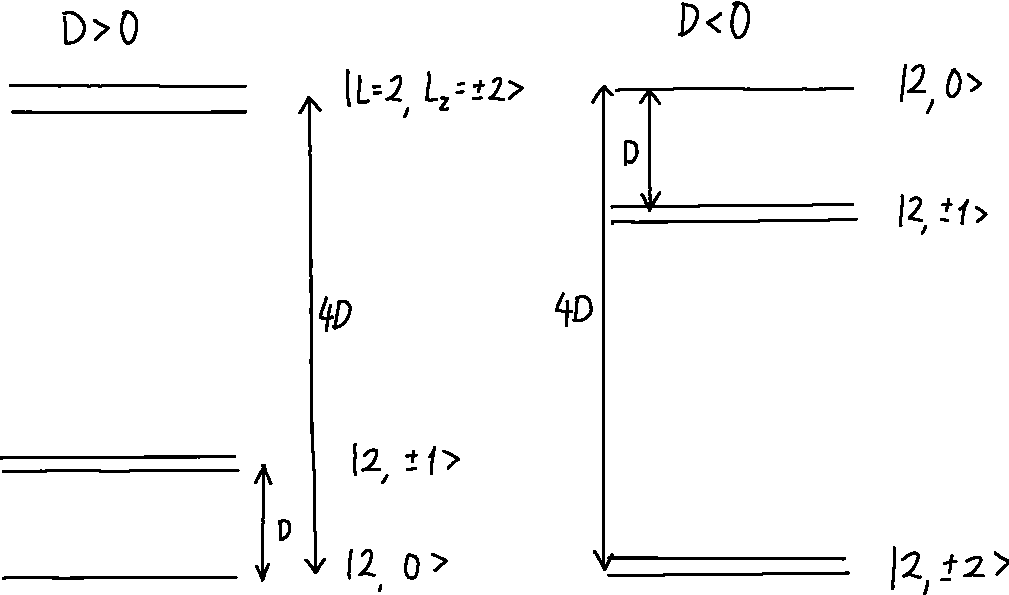
\includegraphics[width=.8\linewidth]{q6-energy-levels}
	\end{figure}
	
	\part Spin-orbit Hamiltonian: $\mathcal{H}_\textnormal{SO} = \lambda \mathbf{L} \cdot \mathbf{S}$, $\lambda < 0$ and $\abs{\lambda} \ll \abs{D}$ so perturb from the crystal field.
	
	For $L = 2$, $S = \diagfrac{1}{2}$, Wigner-Eckart gives $\left\langle\mathbf{L} \cdot \mathbf{S}\right\rangle \propto L_z S_z$ so for the lowest orbital term:
	\begin{figure}[H]
		\centering
		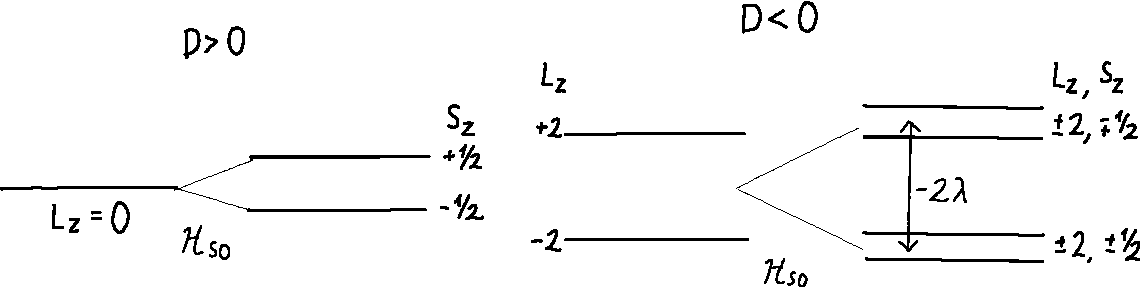
\includegraphics[width=.8\linewidth]{q6-spin-orbit-splitting}
	\end{figure}
	
	\part Zeeman Hamiltonian:
	\begin{align*}
		\mathcal{H}_\textnormal{Z} &= -\mathbf{\mu} \cdot \mathbf{B} \\
		&= \bohrmagneton  \rbracket{\mathbf{L} \cdot \mathbf{B} + 2\mathbf{S} \cdot \mathbf{B}}
	\end{align*}
	
	Since we are further perturbing from the previous interactions, we have:
	\begin{equation*}
		\bohrmagneton  \rbracket{\mathbf{L} \cdot \mathbf{B}} + 2\bohrmagneton  \rbracket{\mathbf{S} \cdot \mathbf{B}} =
		\begin{cases}
			\bohrmagneton  \rbracket{L_z B + 2S_z B} \hspace{1em} \mathbf{B}\parallel\hat{\mathbf{z}} \\
			\bohrmagneton  \rbracket{\underbracket{L_x}_{\frac{L_+ + L_-}{2}} B + 2 \underbracket{S_x}_{\frac{S_+ + S_-}{2}} B} \hspace{1em} \mathbf{B}\bot\hat{\mathbf{z}}
		\end{cases}
	\end{equation*}
	choosing $x$ axis by isotropy.
	
	So for the $\parallel$ case, we have a Zeeman shift of:
	\begin{itemize}
		\item \underline{$D > 0$}
		\begin{equation*}
			\Delta E_z = \pm \bohrmagneton  B \textnormal{\hspace{1em}for\hspace{1em}} \ket{L_z = 0, S_z = \pm\diagfrac{1}{2}}
		\end{equation*}
		\item \underline{$D < 0$}
		\begin{equation*}
			\Delta E_z = \pm \bohrmagneton  B \rbracket{2+1} = \pm 3 \bohrmagneton  B \textnormal{\hspace{1em}for\hspace{1em}} \ket{L_z = \pm 2, S_z = \pm\diagfrac{1}{2}}
		\end{equation*}
	\end{itemize}
	
	For the $\bot$ case, we have:
	\begin{itemize}
		\item \underline{$D > 0$}
		\begin{gather*}
			\begin{split}
				\Delta E_z = \frac{1}{2} &\rbracket{\bra{L_z = 0, S_z = +\diagfrac{1}{2}} + \bra{L_z = 0, S_z -\diagfrac{1}{2}}} \\
				&\mathcal{H}_\textnormal{Z} \\
				&\rbracket{\ket{L_z = 0, S_z = +\diagfrac{1}{2}} + \ket{L_z = 0, S_z = -\diagfrac{1}{2}}}
			\end{split} \\
			\begin{split}
				= &\frac{1}{2} \rbracket{\bra{\ldots} + \bra{\ldots}}
				\sbracket{\bohrmagneton  B \cdot 2 \cdot \frac{1}{2} \sqrt{\diagfrac{1}{2} (\diagfrac{3}{2}) - \diagfrac{1}{2} (\diagfrac{1}{2})} \ket{0, -\diagfrac{1}{2}} \right. \\
				&\left. + \bohrmagneton  B \cdot 2 \cdot \frac{1}{2} \sqrt{\diagfrac{1}{2} (\diagfrac{3}{2}) - (-\diagfrac{1}{2}) (\diagfrac{1}{2})} \ket{0, +\diagfrac{1}{2}}}
			\end{split} \\
			= \frac{1}{2} \sbracket{B \bohrmagneton  + \bohrmagneton  B} = \bohrmagneton  B
		\end{gather*}
		\item \underline{$D < 0$}
		\begin{align*}
			\Delta E_z &= \frac{1}{2} \rbracket{\ldots} \sbracket{\bohrmagneton  B \cdot \frac{1}{2} \sqrt{2 \cdot 3 - (-2) + \ldots} \ket{\ldots} + \ldots} \\
			&= 0 \textnormal{\hspace{1em}since we have no bras with $L_z = \pm 1$}
		\end{align*}
	\end{itemize}
	
	At saturation, we have all moments pointing in the same direction.
	Picking the new ground states then gives:
	\begin{align*}
		D < 0 &\Rightarrow \begin{cases}
			\parallel:\; \mathbf{\mu}_\textnormal{sat} = -\bohrmagneton  \hat{\mathbf{z}} \\
			\bot:\; \mathbf{\mu}_\textnormal{sat} = +\bohrmagneton  \hat{\mathbf{z}}
		\end{cases} \Rightarrow g_\parallel = -\frac{1}{2} \qquad g_\bot = +\frac{1}{2} \\
		D > 0 &\Rightarrow \begin{cases}
			\parallel:\; \mathbf{\mu}_\textnormal{sat} = -3\bohrmagneton  \hat{\mathbf{z}} \\
			\bot:\; \mathbf{\mu}_\textnormal{sat} = 0
		\end{cases} \Rightarrow g_\parallel = -\frac{3}{2} \qquad g_\bot = 0
	\end{align*}
	
	\part An EPR experiment applies an RF pulse to the ion to look for the absorption spectra.
	At transition frequencies, there would be absorption peaks and they may be used to infer the energy levels.
	(Hence the Zeeman splitting too.)
	
	For $D < 0$, since $\mathbf{\mu}_\textnormal{sat} = 0 \bot \hat{\mathbf{z}}$, the splitting at such direction will be unobservable.
\end{parts}